\documentclass[paper=a4, fontsize=11.0pt, abstractoff, DIV12]{scrartcl}
\usepackage[utf8]{inputenc}
\usepackage[ngerman]{babel} % deutsche Rechtschreibung

\usepackage{graphicx} % Grafiken einbinden
\usepackage{amsmath} % AMS! Wichtig!
\usepackage{amsfonts} % mehr AMS
\usepackage{amssymb} % noch viel mehr
\usepackage[amssymb]{SIunits} % Einheiten anständig setzen
\usepackage{bbm} % fetter gedrucktes verfügbar machen, z.B. \mathbbm{1} = Eins mit Doppelstrich
\usepackage[Euler]{simpleMath}
\usepackage{tikz}
\usepackage{hyperref}
\hypersetup{colorlinks,
            breaklinks=true,
            linkcolor=black,
            urlcolor=black,
            citecolor=black,
            bookmarksnumbered,
            pdfauthor={Alexander Eberspächer},
            pdftitle={Seminar Theoretische Physik}}


% define cool colorbox. two arguments: one for title (in bold), the other for the box content.
% Define box and box title style
\tikzstyle{mybox} = [draw=black, fill=white, thin,
    rectangle, rounded corners, inner sep=1ex, inner ysep=2.2ex]
\tikzstyle{fancytitle} =[fill=white, text=black]

\newcommand{\cbox}[2]{
\begin{center}

\begin{tikzpicture}
\node [mybox] (box){%
    \begin{minipage}{0.95\textwidth}
        #2
    \end{minipage}
};
\node[fancytitle, right=1em] at (box.north west) {\textbf{\textsf{#1}}};
\end{tikzpicture}%
\end{center}
} % end newcommand

\title{Crashkurs: Methode der Greenschen Funktion}
\author{Alexander Eberspächer}
\date{\today}

\newcommand{\xhom}{\ensuremath{x_\mathrm{hom}}}
\newcommand{\xinhom}{\ensuremath{x_\mathrm{part}}}
%\newcommand{\Dt}{
\DeclareMathOperator{\Dt}{\mathcal{D}_t}

\begin{document} \maketitle \begin{abstract} Zur Lösung inhomogener
Differentialgleichungen wird die Methode der Greenschen Funktion ohne
Strenge eingeführt. Nach einer kurzen Besprechung von
Fourier-Transformation und Delta-Distribution als notwendiges Handwerkszeug
wird anhand des gedämpften harmonischen Oszillators der Methode vorgestellt.
Ziel ist es, in diesem ersten Kontakt im dritten Semester die Idee hinter
Greenschen Funktionen an einem bekannten Beispiel zu illustrieren.\\[0.5ex]
Literatur: Kuypers \cite{Kuypers}, Arfken\&Weber \cite{Arfken}
\end{abstract}


\section{Einleitung - Worum geht es?}

Beliebige lineare Differentialgleichungen für die Funktion $x = x(t)$
\begin{equation}
f\left(x(t), \dot{x}(t), \dots, x^{(n)}, t\right) = g(t)
\end{equation}
mit linearem $f$ können wir nach den Begriffen \emph{homogen} und \emph
{inhomogen} kategorisieren. Bei homogen Differentialgleichungen ist die
rechte Seite $g(t) = 0$, wohingegen sie für inhomogene
Differentialgleichungen ungleich $0$ ist. Die Lösung für eine inhomogene
Gleichung ist die Summe der Lösung $\xhom(t)$ der homogenen Gleichung und
der partikulären Lösung $\xinhom(t)$ der inhomogenen Gleichung.

Im Folgenden soll illustriert werden, wie man durch die Linearität der
Differentialgleichung aus einer bekannten Lösung für eine ganz bestimmte
Inhomogenität $g(t)$ eine Lösung für \emph{beliebige} Inhomogenitäten
konstruieren kann. Dafür werden wir als Hilfsmittel die
Fourier-Transformation sowie (als die spezielle Inhomogenität) die Delta-
\glqq Funktion\grqq~benötigen, die kurz vorgestellt werden sollen.

\section{Erinnerung: Fourier-Transformation}

\subsection{Fourier-Reihen}

Auf einem Intervall $[-T/2; +T/2]$ periodische Funktionen $x(t)$
lassen sich in eine sogenannte Fourierreihe entwickeln:
\begin{equation}
x(t) = \frac{a_0}{2}+\sum\limits_{n=1}^{\infty}a_n\cos(nx) + \sum\limits_{n=1}^{\infty}b_n\sin(nx)\,,
\end{equation}
wobei die Entwicklungskoeffizienten (Amplituden der \glqq Obertöne\grqq)
$a_n$ und $b_n$ durch
\begin{align}
a_n &:= \frac{2}{T}\int\limits_{-T/2}^{+T/2}x(t)\cos(nx)\,\dd x\\
b_n &:= \frac{2}{T}\int\limits_{-T/2}^{+T/2}x(t)\sin(nx)\,\dd x
\end{align}
mit $n=0,1,2,\dots$ gegeben sind. Diese beiden Gleichungen dürfen Sie als
Skalarprodukt/Projektion lesen: \glqq wie viel $x(t)$ entfällt auf die
Basisfunktionen $\sin(nx)$ beziehungsweise $\cos(nx)$?\grqq

Mit Hilfe der Eulerformel $\eto{\ii\phi}=\cos(\phi)+\ii\sin(\phi)$ ergibt
sich die komplexe Darstellung
\begin{equation}
x(t) = \sum\limits_{n=-\infty}^{+\infty}c_n\eto{\ii n t}
\end{equation}
mit den Entwicklungskoeffizienten
\begin{equation}
c_n := \frac{1}{T}\int\limits_{-T/2}^{+T/2}x(t)\eto{-\ii n t}\,\dd t\,.
\end{equation}

\subsection{Fourier-Transformation}

Gutmütige Funktionen, die nicht periodisch sind, lassen sich im Rahmen eines
Grenzübergangs $T\to\infty$ durch ihre sogenannte Fouriertransformierte
$\tilde x(\omega)$ darstellen gemäß der Gleichung
\begin{equation}
x(t) = \frac{1}{2\pi}\int\limits_{-\infty}^{+\infty} \tilde x(\omega) \eto{\ii \omega t}\,\dd\omega\,,
\label{eq:IFT}
\end{equation}
wobei die Fourier-konjugierte Variable $\omega$ eine Frequenz ist. Die
Fouriertransformierte
\begin{equation}
\tilde x(\omega) := \int\limits_{-\infty}^{+\infty}x(t) \eto{-\ii \omega t}\,\dd t
\label{eq:FT}
\end{equation}
beschreibt dabei im Sinne einer Projektion auf eine Basis nichts anderes als
den Anteil der Funktion $x$, der auf die Frequenz $\omega$ entfällt.
Beachten Sie, dass es viele verschiedene Konventionen für die
Fourier-Transformation gibt (Normierung und Frequenz/Kreisfrequenz).\footnote
{Welche davon benutzt wird ist für die meisten Zwecke ohne Belang, solange
eine Konvention \emph{konsistent} verwendet wird.}

Die Fourier-Transformation ist von herausragender Bedeutung
für viele Probleme der Physik -- so lassen sich beispielsweise
Differentialgleichungen vereinfachen, indem die Relation
\[ \dot x(t) \stackrel{\FT}{\longrightarrow} \ii\omega \tilde x (\omega)\]
ausgenutzt wird. In der Quantenmechanik begegnet uns die Unschärferelation der
Fouriertransformation $\sigma_x \sigma_k \ge 1/2$ (mit den
Standardabweichungen $\sigma_{\{x,k\}}$ als Maß für der Breite der
Verteilungen $f(x)$ beziehungsweise $\tilde f(k)$) mit der
de-Broglie-Beziehung $p=\hbar k$ als Heisenbergsche Unschärferelation
$\sigma_x \sigma_p \ge \hbar/2$ wieder.

Verschiedene Fouriertransformierte finden Sie tabelliert, beispielsweise in
\cite{Gradshteyn}.


\section{Wie modelliert man einen Hammerschlag? - Die Delta-\glqq Funktion\grqq}

\subsection{Was passiert bei einem Hammerschlag? Was ist eine Punktladung?}

Ein idealisierter Hammerschlag überträgt während eines einzigen Zeitpunktes
$t_0$ einen bestimmten Impuls $\Delta p$ auf einen Körper. Nach $F=\dot{p}$
beziehungsweise $F\Delta t = \Delta p$ erwartet man für eine gegen Null
strebende Kontaktzeit $\Delta t$ also eine unendlich große Kraft. Das
mathematische Konstrukt, das die Eigenschaft hat, unter einem Integral
einen bestimmten Wert zu liefern, obwohl es überall außer bei $t=t_0$ gleich
$0$ ist, werden wir die $\delta$-Funktion nennen. Für unseren Hammerschlag
zum Zeitpunkt $t_0$ schreiben wir
\begin{equation}
F = \Delta p \delta(t-t_0)\,.
\end{equation}

Obwohl es sich bei der $\delta$-\glqq Funktion\grqq eigentlich um eine
sogenannte \emph{Distribution} oder \emph{verallgemeinerte Funktion}
handelt, werden wir hier sehr lax von \emph{Funktion} sprechen.

\subsection{Definierende Eigenschaft der Delta-Funktion}

Wir definieren die Delta-Funktion durch folgende Eigenschaft:
\begin{equation}
\int\limits_{-\infty}^{+\infty} \delta(t-t_0) f(t) \,\dd t = f(t_0)\,;
\label{eq:Abtast}
\end{equation}
diese sogenannte Abtasteigenschaft bedeutet, dass ein Integral über ein
Produkt von einer Testfunktion $f(t)$ und der Delta-Funktion $\delta(t-t_0)$
gerade den Funktionswert $f(t_0)$ an der Nullstelle $t_0$ des Arguments der
Delta-Funktion ergibt.

Insbesondere ist mit $f(x) \equiv 1$ die Fläche unter der Delta-Funktion
\begin{equation}
\int\limits_{-\infty}^{+\infty} 1 \,\delta(t)\,\dd t = 1
\end{equation}
gerade gleich $1$.

Analog zum Hammerschlag schreiben wir für die Ladungsdichte, die zu einer
punktförmigen Ladung $q$ am Ort $\vec r_0$ gehört
\begin{equation}
\rho(\vec r) = q \delta^3(\vec r - \vec r_0)\,,
\end{equation}
wobei $\delta^3$ die Delta-Funktion in drei Dimensionen bezeichnet. Das
Integral
\begin{equation}
Q = \int_{\Reals^3}\!\dd V \rho(\vec r)
\end{equation}
über den gesamten Raum ergibt dann die korrekte Gesamtladung $q$.

\subsection{Darstellungen der Delta-Funktion}

Die Delta-Funktion kann als Grenzwert $\lim_{\epsilon}\delta_\epsilon(t -
t_0) = \delta(t-t_0)$ einer Funktionenfolge $\delta_\epsilon$ verstanden
werden. Die Visualisierung dieser Folgen dient der Anschauung. Rechnungen mit
der Delta-Funktion können mit Hilfe dieser Darstellungen gemacht werden,
indem Grenzwert-Bildung und Integration vertauscht werden.

Mögliche Darstellungen sind beispielsweise
\begin{description}
    \item[Rechteck] Das Rechteck
    \begin{equation}
    \delta_\epsilon(t-t_0) = \left\{\begin{array}{l l}\frac{1}{\epsilon} & \qquad t_0-\frac{\epsilon}{2} < t < t_0+\frac{\epsilon}{2}\\ 0 &\qquad\mathrm{sonst}\end{array}\right.
    \end{equation}
    der Breite $\epsilon$ und Höhe $1/\epsilon$ hat die Fläche $1$. Im Limes
    $\lim\limits_{\epsilon\to0}\delta_\epsilon$ ergibt sich die
    Delta-Funktion.

    \item[Gauß] Die Gauß-Glockenkurve
    \begin{equation}
    \delta_\epsilon(t-t_0) = \frac{1}{\sqrt{2\pi}\epsilon} \eto{-(t-t_0)^2/2\epsilon^2}
    \end{equation}
    mit Breite (Standardabweichung) $\epsilon$ ist ebenfalls auf die Fläche
    $1$ normiert. Im Limes $\epsilon \to 0$ geht dann hier auch die Breite
    gegen $0$, wohingegen die \glqq Höhe\grqq~der Glocke gegen $\infty$
    strebt.
    \item[Lorentz] Bei der Lorentz-Kurve
    \begin{equation}
    \delta_\epsilon(t-t_0) = \frac{1}{\pi}\frac{\epsilon}{(t-t_0)^2 + \epsilon^2}
    \end{equation}
    ist $\epsilon$ ebenfalls ein Maß für die Breite. Der relevante Limes ist
    analog zur Gauß-Glocke.
    \item[Sinc] Die Sinc-Funktion
    \begin{equation}
    \delta_\epsilon(t-t_0) = \frac{1}{\epsilon} \frac{\sin((t-t_0)/\epsilon)}{t-t_0}
    \end{equation}
    ist ebenfalls im selben Limes eine Darstellung der Delta-Funktion.
\end{description}
    Die folgende Abbildung illustriert die verschiedenen Darstellungen
    mit verschiedenen Werten für $\epsilon$.
    \begin{center}
        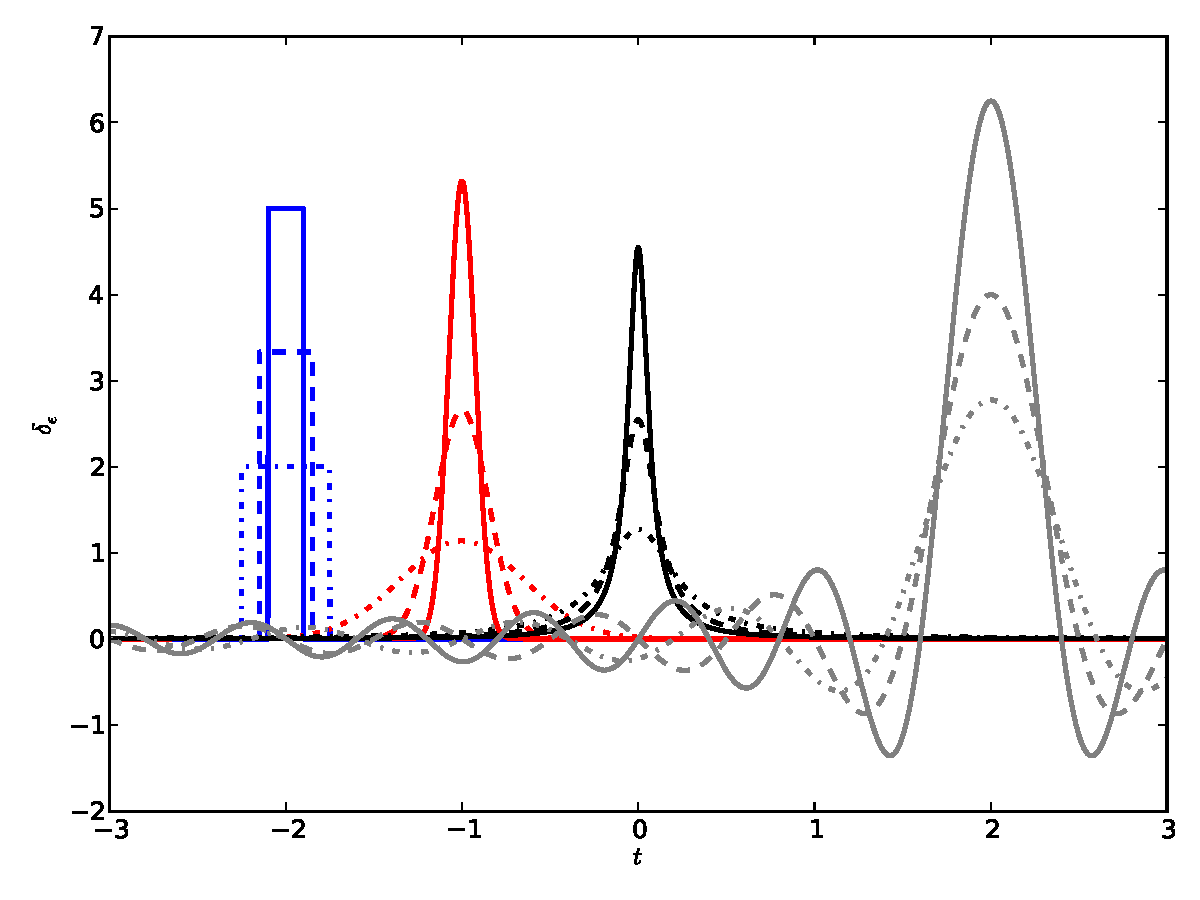
\includegraphics[width=0.7\textwidth]{delta-plot.pdf}
    \end{center}
    Von links nach rechts sind Rechteck-, Gauß-, Lorentz- und
    Sinc-Darstellungen geplottet.


\subsection{Fourier-Darstellung der Delta-Funktion}

Später wird die Fourier-Darstellung der Delta-Funktion von Bedeutung sein.
Um diese zu erhalten, benutzen wir die Fourier-Darstellung \eqref{eq:IFT}
einer Funktion $x(t)$ und setzen in diese die Fourier-Transformierte $\tilde
x(\omega)$ aus \eqref{eq:FT} ein und erhalten
\begin{equation}
x(t) = \frac{1}{2\pi}\int\limits_{-\infty}^{+\infty}\!\dd\omega \left( \int\limits_{-\infty}^{+\infty}\!\dd t' x(t') \eto{-\ii\omega t'} \right) \eto{\ii \omega t}\,,
\end{equation}
oder nach Vertauschen der Integrationsreihenfolge
\begin{equation}
x(t) = \int\limits_{-\infty}^{+\infty}\!\dd t' \left( \int\limits_{-\infty}^{+\infty}\!\frac{\dd\omega}{2\pi} 1\cdot\eto{\ii \omega (t-t')} \right)x(t')\,.
\end{equation}
Der Term in Klammern sorgt genau für das, was wir von Delta-Funktion
$\delta(t-t')$ erwarten -- das $t'$-Integral über $\delta \cdot
\mathrm{Testfunktion}$ ergibt gerade den Wert der Testfunktion an der
Nullstelle $t'=t$ des Arguments der Delta-Funktion. Wir haben also durch
diese Identifikation für die Delta-Funktion die Fourier-Darstellung
\begin{equation}
\delta(t-t') = \frac{1}{2\pi} \int\limits_{-\infty}^{+\infty}\!{\dd\omega}\, 1\cdot\eto{\ii \omega (t-t')}
\label{eq:DeltaFT}
\end{equation}
gefunden. Diese Gleichung kann man auch so lesen, dass die Delta-Funktion
und die konstante Funktion $1$ ein Fourier-Pärchen bilden. Beachten Sie
hier, dass dieses Pärchen auf extreme Art und Weise das Unschärfe-Prinzip
illustriert: in der Frequenz-Domäne tragen hier alle Frequenzen $\omega$
gleichermaßen bei (Gewicht $1$), was eine perfekte Lokalisierung  bei $t=t'$
in der Zeit-Domäne zur Folge hat.

\subsection{*Ausflug: die Fourier-Transformierte von $\cos(\omega_0 t)$}

Als kleinen Ausflug nutzen wir die Fourier-Darstellung der Delta-Funktion,
um explizit ein Fourier-Pärchen zu berechnen.
Wir nutzen die Eulerformel und schreiben
\begin{equation}
\cos(\omega_0 t) = \frac{1}{2}\left(\eto{+\ii\omega_0t} + \eto{-\ii\omega_0 t}\right)\,.
\end{equation}
Fouriertransformation beider Seiten dieser Gleichung führt auf
\begin{equation}
\FT\{\cos(\omega_0t)\} = \frac{1}{2} \int\limits_{-\infty}^{+\infty}\!\dd t\, \eto{-\ii\omega t}\left( \eto{+\ii\omega_0 t}+\eto{-\ii\omega_0 t}\right)\,,
\end{equation}
woraus wir mit \eqref{eq:DeltaFT} schließlich durch Umbennen $\omega
\leftrightarrow t$
\begin{equation}
\FT\{ \cos(\omega_0 t) \} = \pi(\delta(\omega-\omega_0) + \delta(\omega+\omega_0))\,.
\end{equation}
berechnen.


\section{Erzwungene Schwingungen und die Greensche Funktion}

\subsection{Die Differentialgleichung}

Wir sind jetzt gerüstet, unser eigentliches Problem anzugehen -- die erzwungene
Schwingung
\begin{equation}
\ddot{x} + \gamma\dot{x} + \frac{k}{m}x = f(t)\,,
\end{equation}
in der $\gamma \dot{x}$ eine geschwindigkeitsabhängige Reibungskraft,
$\omega_0 = \sqrt{k/m}$ die Frequenz der ungedämpften Schwingung und $f(t)$
eine zeitabhängige treibende Kraft ist. Diese Differentialgleichung ist linear
und inhomogen. Die Lösung schreiben wir als
\begin{equation}
x(t) = \xhom(t) + \xinhom(t)
\label{eq:Sol}
\end{equation}
und definieren etwas formal den Differentialoperator
\begin{equation}
\Dt = \secondderiv{}{t} + \gamma\firstderiv{}{t} + \frac{k}{m}
\end{equation}
mit dem wir die homogene Gleichung als
\begin{equation}
\Dt \xhom(t) = 0
\end{equation}
und die inhomogene Gleichung als
\begin{equation}
\Dt \xinhom(t) = f(t)
\end{equation}
schreiben können. Dass das behauptete $x(t)$ aus \eqref{eq:Sol} tatsächlich
eine Lösung der inhomogenen Differentialgleichung ist zeigen wir, indem wir
$\Dt$ auf $x(t)$ anwenden:
\begin{equation}
\Dt x(t) = \underbrace{\Dt \xhom(t)}_{=0} + \underbrace{\Dt \xinhom(t)}_{=f(t)} = f(t)\,.
\end{equation}
Für die homogene Lösung ergibt sich im Fall \glqq schwacher Dämpfung\grqq~(
$\gamma < 2\omega_0)$ mit $\omega = \sqrt{\omega_0^2 - \gamma/4}$ die
exponentiell ausdämpfende Lösung
\begin{equation}
\xhom(t) = A \eto{-(\ii \omega + \gamma/2)t}\,,
\end{equation}
weshalb nach einiger Zeit nur noch die partikuläre Lösung von Interesse sein
wird.

\subsection{Taktik zur Berechnung der partikulären Lösung}

Als Taktik werden wir die Differentialgleichung zunächst für einen einzelnen
Delta-Kraftstoß mit Einheits-Impulsübertrag lösen. Diese Lösung, die
sogenannte \emph{Greensche Funktion} oder \emph{Fundamentallösung} werden
wir dann nutzen, um für beliebige (!) Inhomogenitäten eine Lösung der
Differentialgleichung anzugeben.

\subsubsection{Erster Schritt: Zerlegung der Inhomogenität}

Wir zerlegen die Inhomogenität $f(t)$ in viele kleine Delta-Kraftstöße:
\begin{equation}
f(t) = \int\limits_{-\infty}^{+\infty}\delta(t-t')f(t')\,\dd t
\end{equation}

\subsection{Zweiter Schritt: Greensche Funktion bestimmen}

Motiviert von der Zerlegung im ersten Schritt lösen wir die
Differentialgleichung nun für einen Einheits-Kraftstoß $\delta(t-t')$. Die
Lösung der Gleichung
\begin{equation}
\Dt G(t-t') = \delta(t-t')
\end{equation}
nennen wir die Greensche Funktion oder die Fundamentallösung. In dieser
steckt die Information darüber, wie das System, das durch $\Dt$ beschrieben
wird auf einen Delta-Kraftstoß antwortet.

\subsubsection{Dritter Schritt: $\xinhom$ zusammenbauen}

Mit der Greenschen Funktion können wir die partikuläre Lösung als
\begin{equation}
\int\limits_{-\infty}^{+\infty} G(t-t') f(t') \,\dd t' = \xinhom(t)
\label{eq:InhomLsg}
\end{equation}
schreiben. Die Gesamtlösung $\xinhom(t)$ erhalten wir, indem wir die
geforderte Linearität der Differentialgleichung ausnutzen und die Lösungen
für gewichtete \glqq Hammerschläge\grqq~$f(t')\delta(t-t')$ zu beliebigen
Zeiten $t'$ superponieren. Um zu zeigen, dass die Behauptung wahr ist,
wenden wir $\Dt$ auf die linke Seite an:
\begin{align}
\Dt \xinhom(t) &= \int\limits_{-\infty}^{+\infty} \underbrace{\Dt G(t-t')}_{=\delta(t-t')} f(t') \,\dd t'\\
&=f(t)\,.
\end{align}

\subsubsection{Anwendung auf die gedämpfte Schwingung}

Mit unserem konkreten $\Dt$ ist also die Gleichung
\begin{equation}
\ddot{G}(t-t') + \gamma\dot{G}(t-t') + \omega_0^2 G(t-t') = \delta(t-t')
\label{eq:GreenDGL}
\end{equation}
zu lösen. Aus einer Differentialgleichung für $\xinhom$ haben wir also eine
Differentialgleichung für $G$ gemacht. Der Aufwand, die nicht ganz triviale
Gleichung \eqref{eq:GreenDGL} zu lösen lohnt insofern, als dass mit
bekanntem $G$ das Problem nach \eqref{eq:InhomLsg} für \emph{beliebige}
Inhomogenitäten $f(t)$ gelöst ist!

Wir werden das Problem mit Hilfe der Fouriertransformation im Frequenz-Raum
lösen. Die Lösung werden wir dann in den Zeit-Bereich zurücktransformieren. Für
eine harmonischen Antrieb können wir alle Integrale analytisch ausführen.

Wir beginnen mit einer Fourierdarstellung der Greenschen Funktion, aus der
wir gleich die benötigten Zeitableitungen berechnen:
\begin{align}
G(t-t') &= \frac{1}{2\pi}\int\limits_{-\infty}^{+\infty} \tilde G(\omega)\eto{\ii\omega(t-t')}\,\dd\omega\\
\leadsto \dot{G}(t-t') &= \ii\omega G(t-t')\\
\leadsto \ddot{G}(t-t') &= -\omega^2 G(t-t')
\end{align}
Das setzen wir nun in \eqref{eq:GreenDGL} ein und erhalten zunächst
\begin{equation}
\frac{1}{2\pi}\int\limits_{-\infty}^{+\infty} \left(-\omega^2 + \ii\omega\gamma + \omega_0^2\right) \tilde G(\omega) \eto{\ii\omega(t-t')}\,\dd\omega = \delta(t-t')\,,
\end{equation}
Wir nutzen nun noch die Fourier-Darstellung der Delta-Funktion \eqref
{eq:DeltaFT} um die rechte Seite umzuschreiben. Wir erhalten
\begin{equation}
\int\limits_{-\infty}^{+\infty} \left(-\omega^2 + \ii\omega\gamma + \omega_0^2\right) \tilde G(\omega) \eto{\ii\omega(t-t')}\,\dd\omega =
\int\limits_{-\infty}^{+\infty} 1 \cdot \eto{\ii\omega(t-t')}\,\dd\omega\,.
\end{equation}
Diese Gleichung ist auf jeden Fall gelöst, wenn die Integranden auf beiden
Seiten gleich sind. Wir erhalten damit für die Greensche Funktion in der
Fourier-Darstellung
\begin{equation}
\tilde G(\omega) =\frac{1}{-\omega^2+\ii\omega\gamma+\omega_0^2}\,.
\end{equation}
Durch Rücktransformation in den Zeit-Bereich finden wir
\begin{equation}
G(t-t') =\frac{1}{2\pi}\int\limits_{-\infty}^{+\infty}\frac{\eto{\ii\omega(t-t')}}{-\omega^2 + \ii\omega\gamma + \omega_0^2}\,\dd\omega\,.
\label{eq:GreenZeit}
\end{equation}
Im Spezialfall der harmonischen treibenden Kraft $f(t) = f_0\eto{\ii\Omega t}$
können wir mit \eqref{eq:GreenZeit} und \eqref{eq:InhomLsg} die partikuläre
Lösung
\begin{equation}
\xinhom(t) = \int\limits_{-\infty}^{+\infty}\!\dd t'\,f_0\eto{\ii\Omega t'} \int\limits_{-\infty}^{+\infty}\!\frac{\dd\omega}{2\pi}\frac{\eto{\ii\omega(t- t')}}{-\omega^2 + \ii\omega\gamma + \omega_0^2}
\end{equation}
berechnen. Wir vertauschen die Integrationsreihenfolge und erhalten mit der
Abtasteigenschaft \eqref{eq:Abtast}
\begin{align}
\xinhom(t) &= \int\limits_{-\infty}^{+\infty}\!{\dd\omega}\frac{f_0 \eto{\ii\omega t}}{-\omega^2 + \ii\omega\gamma + \omega_0^2}\,\underbrace{\frac{1}{2\pi}\int\limits_{-\infty}^{+\infty}\!\dd t' \eto{\ii (\Omega-\omega)t'}}_{=\delta(\Omega-\omega)}\\
&=\frac{f_0}{-\Omega^2 + \ii\Omega\gamma + \omega_0^2}\eto{\ii\Omega t}\,.
\end{align}
Wir machen nun noch den Nenner der Amplitude reell und bilden den Realteil und
erhalten als Endergebnis das schon aus der Vorlesung bekannte Resultat
\begin{equation}
\xinhom(t) = \frac{f_0}{(\omega_0^2 - \Omega^2)^2 + \gamma^2\Omega^2}\cos(\Omega t + \varphi)\,,
\end{equation}
in dem $\varphi$ die (hier nicht explizit angegebene) Phasenverschiebung der Schwingung
ist.

Folgender Plot zeigt nochmals für feste Frequenz $\omega_0$ des ungedämpften
Systems die Abhängigkeit des Amplitudenfaktors von der Frequenz $\Omega$ des
Antriebs für verschiedene Dämpfungen $\gamma$.
\begin{center}
    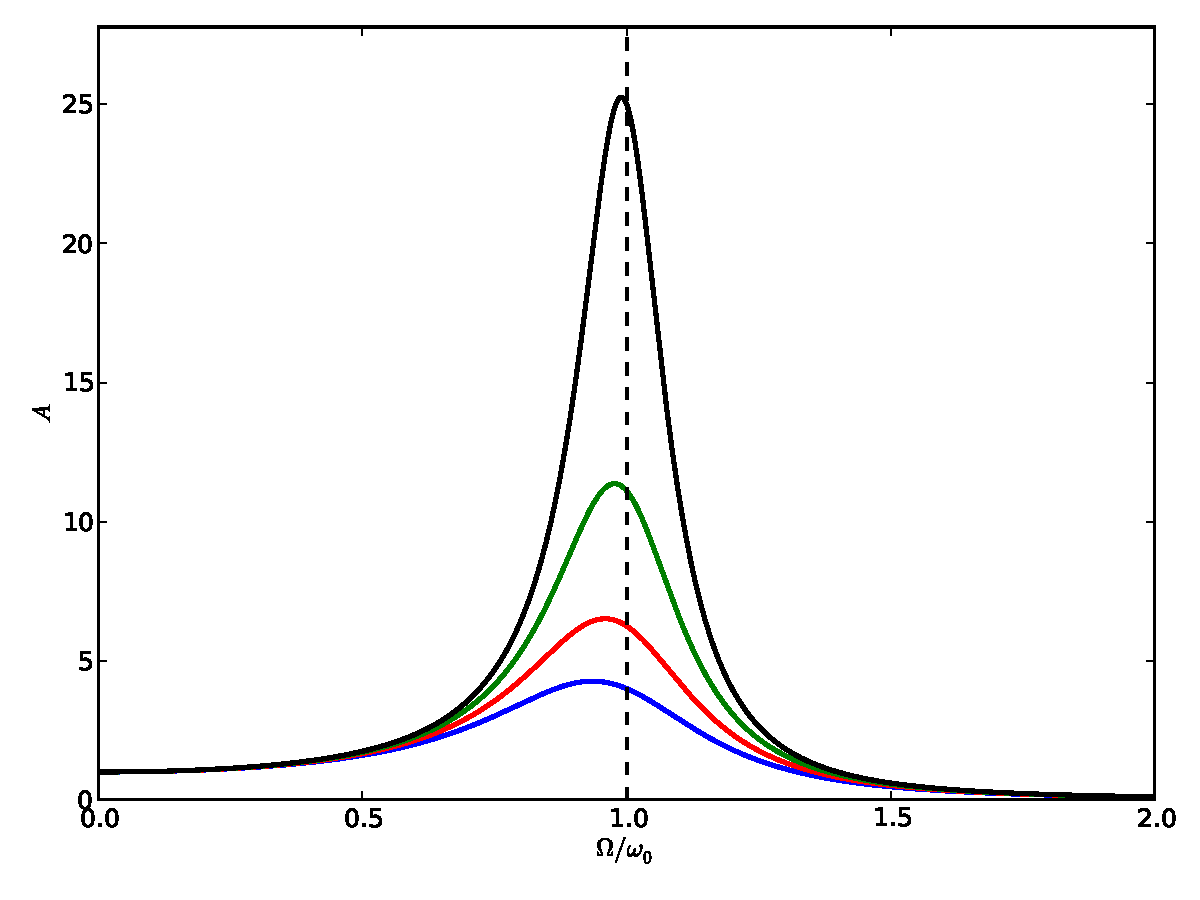
\includegraphics[width=0.7\textwidth]{ampl-plot.pdf}
\end{center}
Höhere Kurven gehören zu kleineren Dämpfungen. Die Maxima der Kurven gehören zu
den jeweiligen Resonanzfrequenzen.


\section{Greensche Funktionen in anderen Gebieten der Physik}

Die Methode der Greenschen Funktion findet in vielen Gebieten der Physik
Anwendung. Eine bestimmte Greensche Funktion ist Ihnen bereits aus der
Schule bekannt (!) -- nämlich die das Laplace-Operators $\Delta$. Sie
wissen, dass sich in der Elektrostatik das elektrische Feld $\vec E(\vec r)$
aus dem Potential $\phi(\vec r)$ gemäß
\begin{equation}
\vec E(\vec r) = - \nabla \phi(\vec r)
\end{equation}
ergibt. Zusammen mit der Maxwell-Gleichung
\begin{equation}
\nabla\cdot\vec E(\vec r) = \frac{\rho(\vec r)}{\epsilon_0}
\end{equation}
ergibt sich als Potentialgleichung die sogenannte Poisson-Gleichung
\begin{equation}
\Delta\phi(\vec r) = -\frac{\rho(\vec r)}{\epsilon_0}\,.
\end{equation}
Nun kennen Sie aus der Schule das Potential einer Punktladung $\rho(\vec r)
= q \delta^3(\vec r - \vec r')$ am Ort $\vec r'$:
\begin{equation}
\phi(\vec r) = \frac{q}{4\pi\epsilon_0}\frac{1}{\abs{\vec r - \vec r'}}
\end{equation}
Durch Einsetzen in die Poisson-Gleichung finden Sie also
\begin{equation}
\Delta\phi(\vec r) = \Delta\left(\frac{q}{4\pi\epsilon_0}\frac{1}{\abs{\vec r - \vec r'}}\right) = -\frac{q}{\epsilon_0} \delta^3(\vec r - \vec r')
\end{equation}
Durch Vergleich dieser Gleichung mit der Definition der Greenschen Funktion
lesen wir die Fundamentallösung für den Laplace-Operator einfach ab
als\footnote{Gelegentlich werden auch Definitionen für mit Minuszeichen für
die Greensche Funktion benutzt.}
\begin{equation}
G(\vec r - \vec r') = -\frac{1}{4\pi}\frac{1}{\abs{\vec r - \vec r'}}\,.
\end{equation}
Für beliebige Ladungsdichten $\rho(\vec r)$ könenn Sie damit analog zu
\eqref{eq:InhomLsg} das Potential $\phi(\vec r)$ berechnen als
\begin{equation}
\phi(\vec r) = -\int\limits_{\Reals^3}\!\dd V'\,\frac{1}{4\pi\epsilon_0}\frac{\rho(\vec r')}{\abs{\vec r - \vec r'}}\,.
\end{equation}
Beachten Sie, dass auf etwaige Komplikationen durch Randbedingungen an dieser
Stelle nicht eingegangen wird.


\bibliographystyle{ieeetr}

\bibliography{Mechanik-GreensFkt}

\end{document}
